\chapter{Background: Namespace Scalability}
\label{chp:related-work}

% what is a global namespace
A namespace organizes data by name. Traditionally, namespaces are hierarchical
and allow users to group similar data together in an unbounded way; the number
of files/directories, the shape of the namespace, and the depth of the
hierarchy are free to grow as large as the user wants~\cite{levy:acm90-survey,
tanenbaum:book05-os, arpaci-dusseau:book14-os}.  Examples include file systems,
DNS, LAN network topologies, and scoping in programming languages.  Because of
this tree-likes structure, we call portions of the namespaces ``subtrees".  The
momentum of namespaces as a data model and the overwhelming amount of legacy
code written for namespaces make the data model relatively future proof.

% file metadata
In this thesis, we focus on file system namespaces.  File system namespaces are
popular because they fit our mental organization as humans and are part of the
POSIX IO standard.  In file systems, whenever a file is created, modified, or
deleted, the client must access the file's metadata. File system metadata
contains information about the file, like size, links, access times,
attributes, permissions/access control lists (ACLs), and ownership.  In single
disk file systems, clients consult metadata before seeking to data, by
translating the file name to an inode and using that inode to lookup metadata
in an inode table located at a fixed location on disk.  Distributed file
systems use a similar idea; clients look in one spot for their metadata,
usually a metadata service, and use that information to find data in a storage
cluster.  State-of-the-art distributed file systems decouple metadata from data
access so that data and metadata I/O can scale
independently~\cite{alam:pdsw2011-metadata-scaling, ghemawat:sosp2003-gfs,
hildebrand:msst2005-pnfs, weil:osdi2006-ceph, welch:fast08-panasas,
xing:sc2009-skyfs}.  Unfortunately, recent trends have shown that separating
metadata and data traffic is insufficient for scaling to large systems and
identify the metadata service as the performance critical component.

First, we describe general file system use cases and
characterize the resultant metadata workloads. Next, we describe three
semantics that users expect from file systems: strong consistency, durability,
and a hierarchical organization.  For each semantic, we explain why it is
problematic for today's metadata workloads and survey optimizations in related
work. We conclude this section by scoping the thesis.

%% general optimization An accepted optimization for distributed file systems
%is to maintain system-specific information about accessing files.  Per-client
%capabilities for a file gives clients opportunities to optimize performance.
%For example, CephFS clients are granted capabilities for reading, reading and
%updating, caching reads, writing, buffering writes, extending the end of a
%file, and doing lazy IO~\cite{docs:cephcaps}; GPFS allows byte range locking
%for writing different parts of a file~\cite{schmuck:fast2002-gpfs}; meanwhile,
%GFS does not let clients cache or buffer data because their applications
%typically stream~\cite{ghemawat:sosp2003-gfs}. Another system-specific piece
%of metadata common in distributed file systems is data location or layout
%information, such as striping strategies~\cite{nagle_panasas_2004,
%welch:fast08-panasas, wang:tech09-lustre, docs:cephstripe,
%sinnamohideen:atc2010-ursa, ghemawat:sosp2003-gfs}. This lets clients contact
%the storage servers for data IO after doing only one RPC to retrieve the map
%of data locations.  Other systems have similar capabilities but are not
%enumerated here because these optimizations are for data IO.  Instead we focus
%on similar optimizations for serving the metadata itself.

\section{Metadata Workloads}

% What is the metadata management problem?
File system workload are made up mostly of metadata requests, which are small
and have locality locality~\cite{roselli:atec2000-FS-workloads,
abad:ucc2012-mimesis, leung:atc08-cifs}.  This skewed workload causes
scalability issues in file systems because solutions for scaling data IO do not
work for metadata IO~\cite{roselli:atec2000-FS-workloads,
abad:techreport2012-fstrace, alam:pdsw2011-metadata-scaling,
weil:osdi2006-ceph}.  Unfortunately, this metadata problem is becoming more
common and the same challenges that plagued HPC systems for years are finding
their way into the cloud at Facebook~\cite{borthakur:website17},
LinkedIn~\cite{xiao:socc15-shardfs}, and Google~\cite{dean_evolution_2010,
mckusick:acm2010-gfs-evolution}.  Jobs that deal with many small files ({\it
e.g.}, log processing and database
queries~\cite{thusoo:sigmod2010-facebook-infrastructure}) and large numbers of
simultaneous clients ({\it e.g.}, MapReduce
jobs~\cite{mckusick:acm2010-gfs-evolution}) are especially problematic.

If the use case is narrow enough, then developers in these domains can build
application-specific storage stacks based on a thorough understanding of the
workloads ({\it e.g.}, temperature zones for
photos~\cite{muralidhar:osdi2014-f4}, well-defined read/write
phases~\cite{dean:osdi2004-mapreduce, dean_evolution_2010}, synchronization
only needed during certain phases~\cite{hakimzadeh:dais14-hdfs-consistency,
zheng:pdsw2015-deltafs}, workflows describing computation~\cite{yoo_slurm_2003,
gamblin_spack_2015}, etc.). Unfortunately, this ``clean-slate" approach only
works for one type of workload. To build a general-purpose file system, we need
a thorough understanding of today's workloads and how they affect metadata
services.  

In this section, we describe modern applications ({\it i.e.} standalone
programs, compilers, and runtimes) and common user behaviors ({\it i.e.} how
users interact with file systems) that result in metadata-intensive workloads.
For each use case, we provide motivation from HPC and cloud workloads;
specifically, we look at users using the file system in parallel to run
large-scale experiments in HPC and parallel runtimes that use the file system,
such as MapReduce~\cite{dean:osdi2004-mapreduce} (referred to as Hadoop, the
open-source counterpart~\cite{shvachko_hadoop_2010}),
Dryad~\cite{isard:EuroSys2007-dryad}, and Spark~\cite{zaharia:nsdi2012-spark}.
We choose these use cases because they are representative of two very different
architectures:  scale-out and scale-up (although the line between scale-up and
out has been blurred recently~\cite{gigaspaces:whitepaper2011-su-vs-so,
michael:2007pdps-scale-up-x-scale-out,
rowstron:hotcdp2012-hadoop-vs-single-node, sevilla:discs2013-framework, 
sevilla:lspp2014-supmr}).

% Locality is a big part of workloads
\subsection{Spatial Locality Within Directories}
\label{sec:spatial-locality-within-directories}

File system namespaces have semantic meaning; data stored in directories is
related and is usually accessed together~\cite{weil:osdi2006-ceph,
weil:sc2004-dyn-metadata}. Programs, compilers, and runtimes are usually
triggered by users so the inputs/outputs to the job are stored within the
user's home directory~\cite{weil:phdthesis07}. Hadoop and Spark enforce POSIX
IO permissions and ownership to ensure users and bolt-on software packages
operate within their assigned directories~\cite{docs:hadoopperm}.  User
behavior also exhibits locality. Listing directories after jobs is common and
accesses are localized to the user's working
directory~\cite{roselli:atec2000-FS-workloads, abad:ucc2012-mimesis}.

A problem in HPC is users unintentionally accessing files in another user's
directory. This behavior introduces false sharing and many file systems revoke
locks and cached items for all clients to ensure consistency. While HPC tries
to avoid these situations with workflows~\cite{zheng:pdsw2014-batchfs,
zheng:pdsw2015-deltafs}, it still happens in distributed file systems when
users unintentionally access directories in a shared file system. 

%Exploiting this locality has positive implications for performance because it
%reduces the number of requests, lowers the communication across metadata server
%nodes, and eases memory pressure.  CephFS tries to leverage this spatial,
%temporal, and request-type locality in metadata intensive workloads using
%dynamic subtree partitioning, but struggles to find the best degree of locality
%and balance.

\subsection{Temporal Locality During Flash Crowds}
\label{sec:temporal-locality-during-flash-crowds}

Creates in the same directory is a problem in HPC, mostly due to
checkpoint-restart~\cite{bent_plfs_2009}. Flash crowds of checkpoint-restart
clients simultaneously open, write, and close files within a directory.  But
the workload also appears in cloud jobs: Hadoop and Spark use the file
\newcomment{system to assign work units to workers and the performance is
proportional to the open/create throughput of the underlying file
system~\cite{xiao:socc15-shardfs, shi:vldb15-spark,
shvachko:login2012-hdfs-scalability}; Big Data Benchmark jobs examined
in~\cite{chaimov:hpdc16-spark} have on the order of 15,000 file opens or
creates just to start a single Spark query and the Lustre system they tested on
did not handle creates well, showing up to a \(24\times\) slowdown compared to
other metadata operations. Common approaches to solve these types of
bottlenecks is to change the application behavior or to design a new file
system, like BatchFS~\cite{zheng:pdsw2014-batchfs} or
DeltaFS~\cite{zheng:pdsw2015-deltafs}, that uses one set of metadata
optimizations for the entire namespace.} \oldcomment{ abstraction to exchange
work units to workers or to indicate when jobs complete  The workload is
clients creating 100K files in private directories in the same global
namespace.} 

\subsection{Listing Directories}
\label{sec:listing-directories}

As discussed before, listing directories is common for general users ({\it e.g.}, reading a
directory after a job completes), but the file system is also used for its
centralized consistency.  For example, users often leverage the file system to
check the progress of jobs using \texttt{ls} even though this operation is
notoriously heavy-weight~\cite{carns:ipdps09-pvfs, eshel:fast10-panache}. The
number of files or size of the files is indicative of the progress. This
practice is not too different from cloud systems that use the file system to
manage the progress of jobs; Spark/Hadoop writes to temporary files, renames
them when complete, and creates a ``DONE" file to indicate to the scheduler that
the task did not fail and should not be re-scheduled on another node.
\newcomment{For example, the browser interface lets Hadoop/Spark users check progress by
querying the file system and returning a \% of job complete metric.} 

\subsection{Performance and Resource Utilization}

\begin{figure}[t]
  \centering
  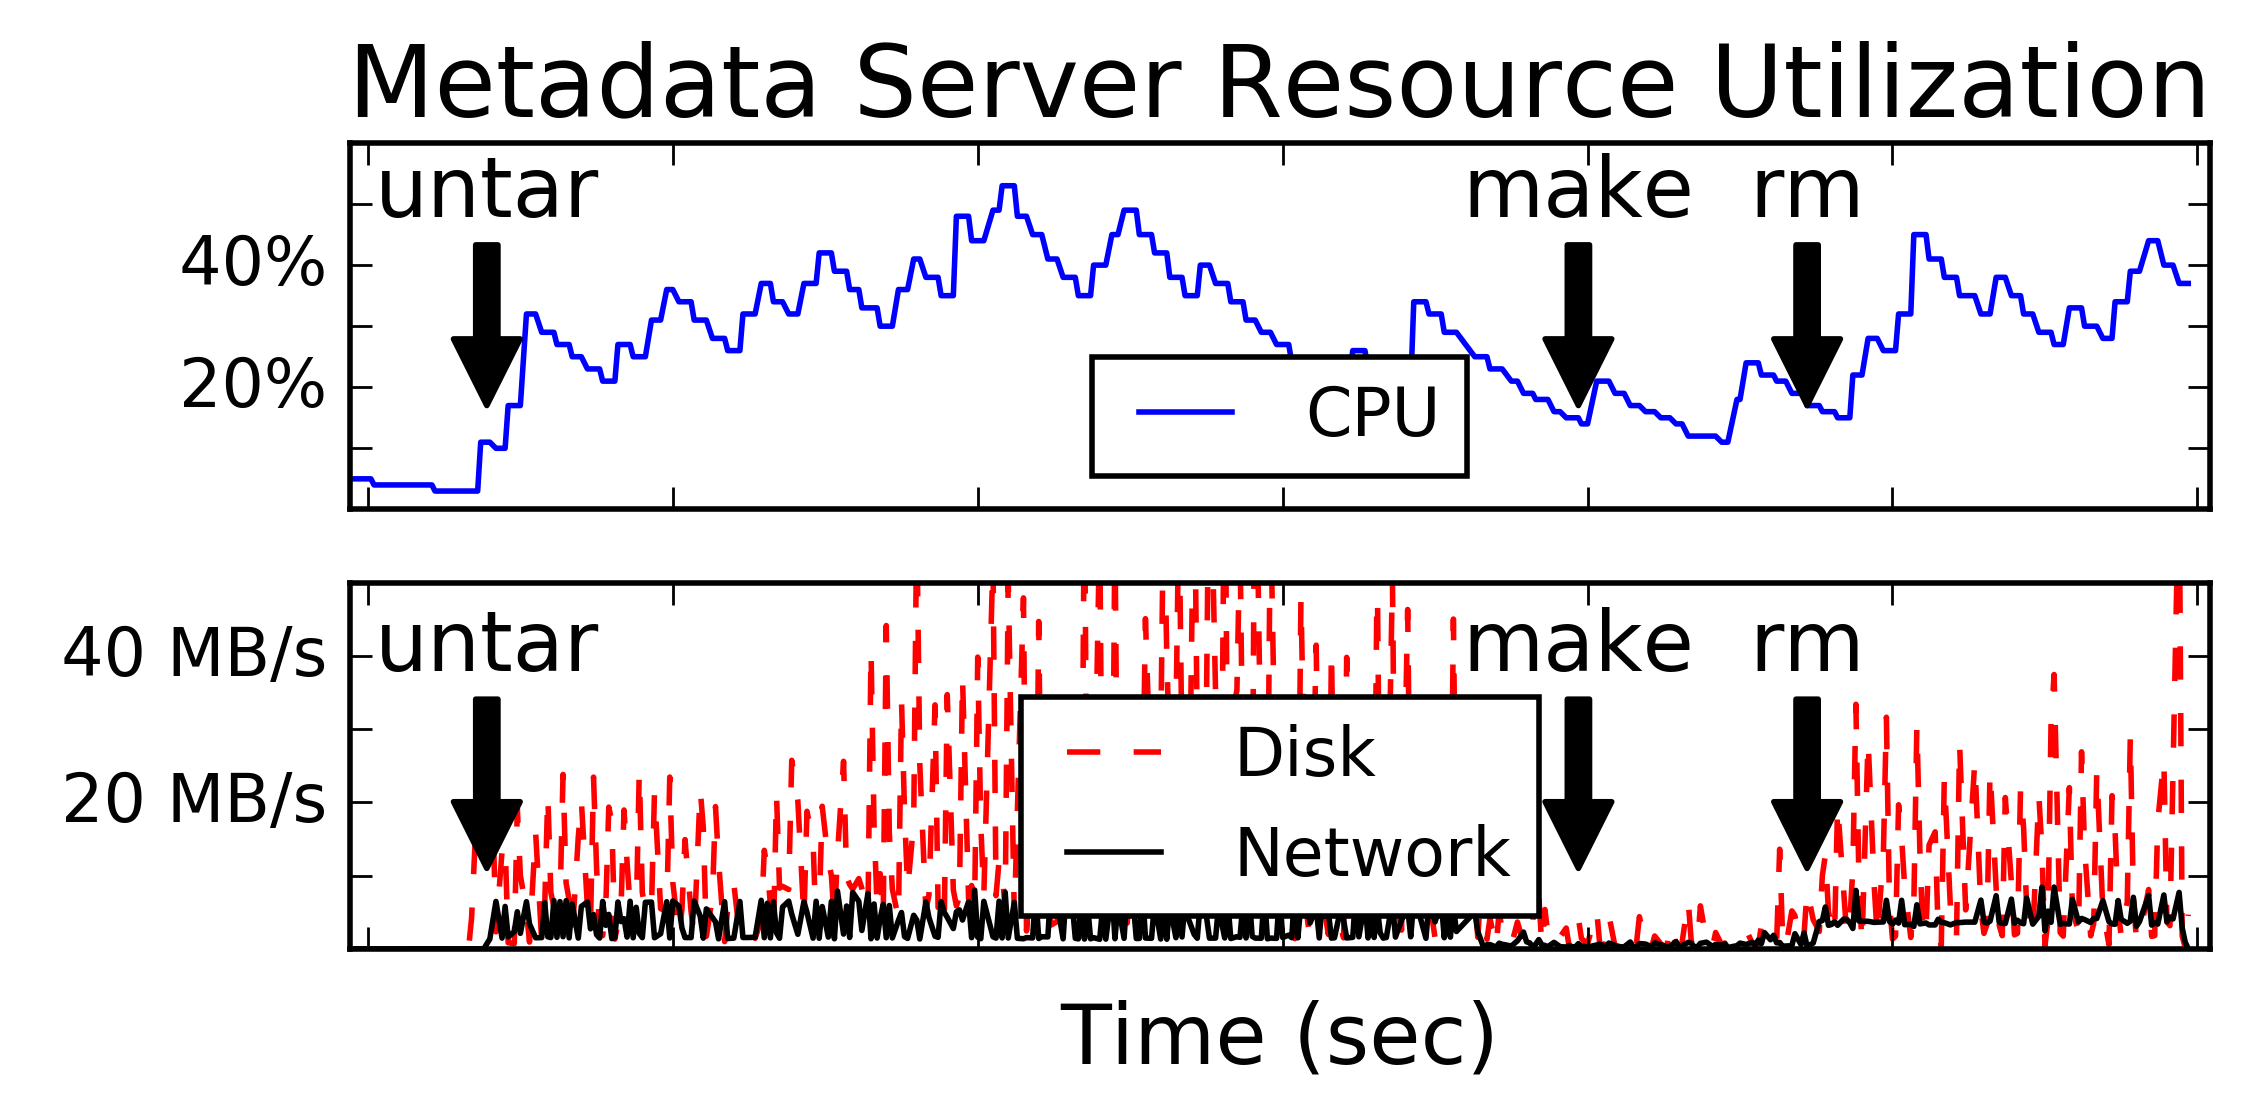
\includegraphics[width=0.7\textwidth]{./chapters/cudele/figures/overhead-creates.png}
  \caption{[\href{https://github.com/michaelsevilla/cudele-popper/blob/master/experiments/baseline-compile/visualize/viz.ipynb}{source}]
  For the CephFS metadata server, create-heavy workloads ({\it e.g.},
  \texttt{untar}) incur the highest disk, network, and CPU utilization because of
  consistency/durability demands.}\label{fig:overhead-creates}
\end{figure}

\begin{figure}[t]
  \centering	
  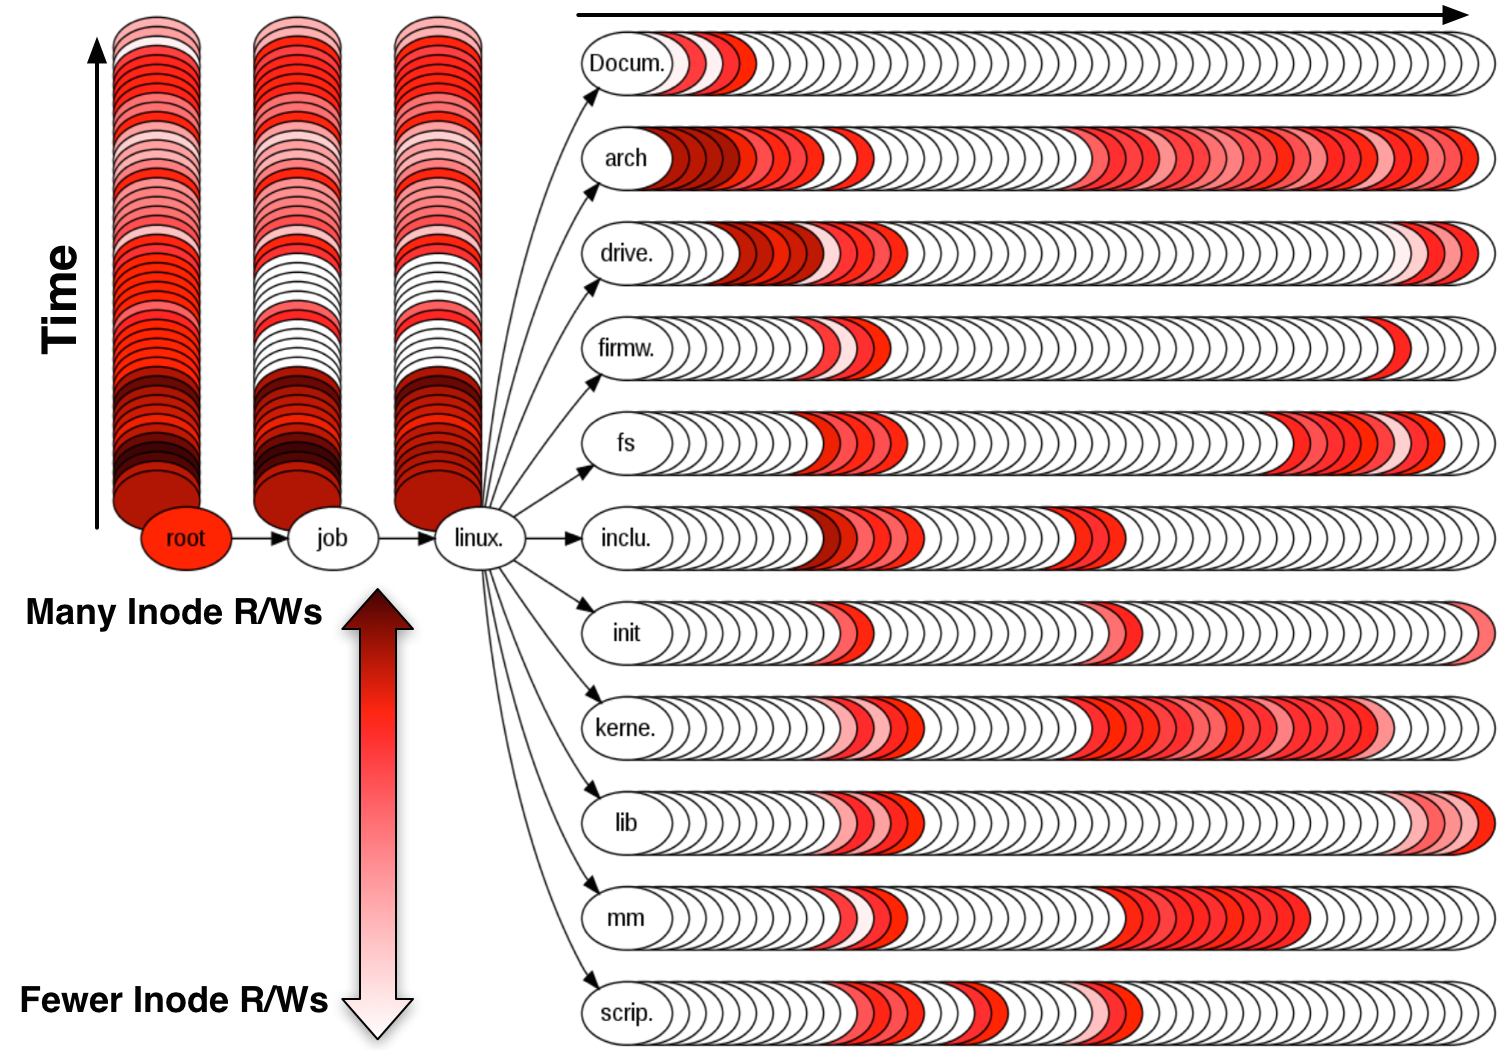
\includegraphics[width=0.7\textwidth]{./chapters/mantle/figures/workload-tar.png}
  \caption{Metadata hotspots, represented by different shades of red, have
  spatial and temporal locality when compiling the Linux source code. The
  hotspots are calculated using the number of inode reads/writes and
  smoothed with an exponential decay. \label{figure:workload-tar}}
\end{figure}

The metadata workloads discussed in the previous section saturate resources on
the metadata servers.  Even small scale programs can show the effect; the
resource utilization on the metadata server when compiling the Linux source
code in a CephFS mount is shown in Figure~\ref{fig:overhead-creates}.  The
\texttt{untar} phase, which is characterized by many creates, has the highest
resource usage (combined CPU, network, and disk) on the metadata server because
of the number of RPCs needed for consistency and durability.  Many of our
benchmarks use a create-heavy workload because it has high resource
utilization.

Figure~\ref{figure:workload-tar} shows the metadata locality for this workload.
The ``heat" of each directory is calculated with per-directory metadata
counters, which are tempered with an exponential decay.  The hotspots can be
correlated with phases of the job: untarring the code has high, sequential
metadata load across directories and compiling the code has hotspots in the
\texttt{arch}, \texttt{kernel}, \texttt{fs}, and \texttt{mm} directories.  

\section{Global Semantics: Strong Consistency}

% what is it
Access to metadata in a POSIX IO-compliant file system is strongly consistent,
so reads and writes to the same inode or directory are globally ordered.  The
benefit of strong consistency is that clients and servers have the same view of
the data, which makes state changes easier to reason about.  The cost of this
``safety" is performance.  The synchronization and serialization machinery
needed to ensure that all clients see the same state has high overhead.  To
make sure that all nodes or processes in the system are seeing the same state,
they must come to an agreement.  This limits parallelization and metadata
performance has been shown to {\it decrease} with more sockets in
Lustre~\cite{konstantinos:pdsw2014-lustre-metadata}. As a result, and because
it is simpler to implement, many distributed file systems limit the number of
threads to one for all metadata servers~\cite{weil:osdi2006-ceph,
alam:pdsw2011-metadata-scaling, ren:sc2014-indexfs}. 

% heavy weight agreement
Agreeing on the state of file system metadata has its own set of performance and accuracy trade-offs.
Sophisticated, standalone consensus engines like
PAXOS~\cite{lamport_parttime_1998}, Zookeeper~\cite{hunt_zookeeper_2010}, or
Chubby~\cite{burrows_chubby_2006} are common techniques for maintaining
consistent versions of state in groups of processes that may disagree, but
putting them in the data path is a large bottleneck. In fact, PAXOS is used in
Ceph and Zookeeper in Apache stacks to maintain cluster state but not for
mediating IO.  

% leases, locks, capabilities
Many distributed file systems use state machines to agree on file system
metadata state.  These state machines are stored with traditional file system
metadata and they enforce the level of isolation that clients are guaranteed
while they are reading or writing a file. CephFS~\cite{docs:cephcaps,
weil:phdthesis07} calls the state machines ``capabilities" and they are managed
by authority metadata servers, GPFS~\cite{schmuck:fast2002-gpfs} calls the
state machines ``write locks" and they can be shared,
Panasas~\cite{welch:fast08-panasas} calls the state machines ``locks" and
``callbacks", IndexFS~\cite{ren:sc2014-indexfs} calls the state machines
``leases" and they are dropped after a timeout,
Lustre~\cite{schwan_lustre_2003} calls the state machines ``locks" and they
protect inodes, extents, and file locks with different modes of
concurrency~\cite{wang:tech09-lustre}.  Because this form of consistency is a
bottleneck for metadata access, many systems optimize performance by improving
locking protocols (Section~\S\ref{sec:lock-management}), caching inodes
(Section~\S\ref{sec:caching-inodes}), and relaxing consistency
(Section~\S\ref{sec:relaxing-consistency}). We refer to these state machines as
``locks" from now.

\subsection{Lock Management}
\label{sec:lock-management}

The global view of locks are usually read and modified with RPCs from clients.  Single
node metadata services, such as the Google File System
(GFS)~\cite{ghemawat:sosp2003-gfs} and
HDFS~\cite{shvachko:login2012-hdfs-scalability} have the simplest
implementations and expose simple lock configurations like timeout thresholds.
These implementations do not scale for metadata-heavy workloads so a natural
approach to improving performance is to use a cluster to manage locks.

% multi node metadata servers
Distributed lock management systems spread the lock request load across a
cluster of servers. One approach is to distribute locks with the data by
co-locating metadata servers with storage servers.
PVFS2~\cite{devulapalli:ipdps07-pvfs2} lets users spin up metadata servers on
both storage and non-storage servers but the disadvantage of this approach is
resource contention and poor file system metadata locality, respectively.
Similarly, the Azure Data Lake Store (ADLS) file
system~\cite{ramakrishnan:sigmod17-adls} stores some types of metadata with
data and some in the centralized metadata store; Microsoft can afford to keep
metadata localized to a single server because they relax consistency semantics
and have a clean-slate file system custom-built for their workloads.  Another
approach is to orchestrate a dedicated metadata cluster from a centralized lock
manager that accounts for load imbalance and locality.
GPFS~\cite{schmuck:fast2002-gpfs} assigns a process to be the ``global lock
manager", which is the authority of all locks and synchronizes access to
metadata. Local servers become the authority of metadata by contacting the
global lock manager, enabling optimizations like reducing RPCs. A decentralized
version of this approach is to associate an authority process per inode. For
example, Lustre, CephFS, IndexFS, and Panasas servers manage parts of the
namespace and respond to client requests for locks.  These approaches have more
complexity but are flexible enough to service a range of workloads.

\subsection{Caching Inodes}
\label{sec:caching-inodes}

The discussion above refers to server-server lock exchange, but systems can
also optimize client-server lock management. Caching inodes on both the client
and server lets clients read/modify metadata locally.  This reduces the number
of RPCs required to agree on the state of metadata.  For example, CephFS caches
entire inodes, Lustre caches lookups, IndexFS caches ACLs, PVFS2 maintains a
namespace cache and an attribute cache, Panasas lets clients read, cache, and
parse directories, GPFS and Panasas cache the results of
\texttt{stat()}~\cite{depardon:tech13-survey}, and GFS caches file
location/striping strategies.  Some systems, like Ursa
Minor~\cite{sinnamohideen:atc2010-ursa} and
pNFS~\cite{hildebrand:msst2005-pnfs} maintain client caches to reduce the
overheads of NFS. These caches improve performance but the cache coherency
mechanisms add significant complexity and overhead for some workloads.

\subsection{Relaxing Consistency}
\label{sec:relaxing-consistency}

% What is HPC doing?
A more disruptive technique is to relax the consistency semantics in the file
system.  Following the models pioneered by Amazon's eventual
consistency~\cite{decandia:sosp2007-dynamo} and the more fine-grained
consistency models defined by Terry et al.~\cite{terry_replicated_2013}, these
techniques are gaining popularity because maintaining strong consistency has
high overhead and because weaker guarantees are sufficient for many target
applications. 

Batching requests together is one form of relaxing consistency because updates
are not seen immediately. PVFS2 batches creates, Panasas combines similar
requests ({\it e.g.}, create and stat) together into one message, and Lustre
surfaces configurations that allow users to enable and disable batching.
Technically, batching requests is weaker than per-request strong consistency
but the technique is often acceptable in POSIX-compliant systems.

More extreme forms of batching ``decouple the namespace", where clients lock
the subtree they want exclusive access to as a way to tell the file system that
the subtree is important or may cause resource contention in the near-future.
Then the file system can change its internal structure to optimize performance.
One software-based approach is to prevent other clients from interfering with
the decoupled directory until the first client commits changes back to the
global namespace. This delayed merge ({\it i.e.} a form of eventual
consistency) and relaxed durability improves performance and scalability by
avoiding the costs of RPCs, synchronization, false sharing, and serialization.
BatchFS and DeltaFS clients merge updates when the job is complete to avoid
these costs and to encourage client-side processing. Another example approach
is to move metadata intensive workloads to more powerful hardware. For example,
for high metadata load MarFS~\cite{grider:pdsw2015-marfs} uses a cluster of
metadata servers and TwoTiers~\cite{bent:slides-twotiers} uses SSDs for the
metadata server back-end.  While the performance benefits of decoupling the
namespace are obvious, applications that rely on the file system's guarantees
must be deployed on an entirely different system or re-written to coordinate
strong consistency themselves.  

Even more drastic departures from POSIX IO allow writers and readers to
interfere with each other. GFS leaves the state of the file undefined rather
than consistent, forcing applications to use append rather than seeks and
writes; in the cloud, Spark and Hadoop stacks use the Hadoop File System
(HDFS)~\cite{shvachko:msst10}, which lets clients ignore this type of
consistency completely by letting interfering clients read files opened for
writing~\cite{hakimzadeh:dais14-hdfs-consistency};
HopsFS~\cite{niaza:fast17-hopsfs}, a fork of HDFS with a more scalable metadata
service, relaxes consistency even further by allowing multiple readers and
multiple writers; ADLS has unique implementations catered to the types of
workloads at Microsoft, some of which have non-POSIX IO APIs; and CephFS offers
the ``Lazy IO" option, which lets clients buffer reads/writes even if other
clients have the file open and if the client maintains its own cache
coherency~\cite{docs:cephcaps}. As noted earlier, many of these relaxed
consistency semantics are for application-specific optimizations.

\section{Global Semantics: Durability}

While durability is not specified by POSIX IO, users expect that files they
create or modify survive failures. The accepted technique for achieving
durability is to append events to a journal of metadata updates.  Similar to
LFS~\cite{rosenblum:acm1992-LFS} and WAFL~\cite{hitz:wtec1994-WAFL} the
metadata journal is designed to be large (on the order of MBs) which ensures
(1) sequential writes into the storage device ({\it e.g.}, object store, local
disk, etc.) and (2) the ability for daemons to trim redundant or irrelevant
journal entries. We refer to metadata updates as a journal, but of course,
terminology varies from system to system ({\it e.g.}, operation log, event
list, etc.). Ensuring durability has overhead so many performance optimizations
target the file system's journal format and mechanisms.

\subsection{Journal Format}

A big point of contention for distributed file systems is not the technique of
journaling metadata updates, rather it is the format of metadata. CephFS
employs a custom on-disk metadata format that behaves more like a ``pile
system"~\cite{weil:phdthesis07}. Alternatively, IndexFS stores its journal in
LSM trees for fast insertion and lookup.  TableFS~\cite{ren:atc2013-tablefs}
lays out the reasoning for using LSM trees: the size of metadata (small) and
the number of files (many) fits the LSM model well, where updates are written
to the local file system as large objects ({\it e.g.}, write-ahead logs,
SSTables, large files). Panasas separates requests out into separate logs to
account for the semantic meaning and overhead of different requests (``op-log"
for creates and updates and ``cap-log" for capabilities).  Many papers claim
that an optimized journal format leads to large performance
gains~\cite{ren:atc2013-tablefs, ren:sc2014-indexfs, zheng:pdsw2014-batchfs}
but we have found that the journal safety mechanisms have a much bigger impact
on performance~\cite{sevilla:ipdps18-cudele}.

\subsection{Journal Safety}

We define three types of durability: global, local, and none.  Global
durability means that the client or server can fail at any time and metadata
will not be lost because it is ``safe" ({\it i.e.} striped or replicated across
a cluster). GFS achieves global durability by replicating its journal from the
master local disk to remote nodes and CephFS streams the journal into the
object store. Local durability means that metadata can be lost if the client or
server stays down after a failure. For example, in BatchFS and DeltaFS
unwritten metadata updates are lost if the client (and/or its disk) fails and
stays down.  None means that metadata is volatile and that the system provides
no guarantees when clients or servers fail.  None is different than local
durability because regardless of the type of failure, metadata will be lost
when components die. Storing the journal in a RAMDisk would be an example of a
system with a durability level of none.

Implementations of the types of durability vary, ranging from completely
software-defined storage to architectures where hardware and software are more
tightly-coupled, such as Panasas. Panasas assigns durability components to
specific types of hardware. The journal is stored in battery-backed NVRAM and
later replicated to both remote peers and metadata on objects. The software
that writes the actual operations behaves similar to WAFL/LFS without the
cleaner. The system also stores different kinds of metadata (system vs. user,
read vs. write) in different places. For example, directories are mirrored
across the cluster using RAID1. This domain-specific mapping to hardware
achieves high performance but sacrifices cost flexibility.

\section{Hierarchical Semantics}

Users identify and access file system data with a path name, which is a list of
directories terminated with a file name.  File systems traverse (or resolve)
paths to check permissions and to verify that files exist. Files and
directories inherit some of the semantics from their parent directories, like
ownership groups and permissions. For some attributes, like access and
modifications times, parent directories must be updated as well. 

% Path traversal
To maintain these semantics, file systems implement path traversal. Path
traversal starts at the root of the file system and checks each path component
until reaching the desired file. This process has write and read amplification
because accessing lower subtrees in the hierarchy requires RPCs to upper
levels. To reduce this amplification, many systems try to leverage the
workload's locality; namely that directories at the top of a namespace are
accessed more often~\cite{ren:sc2014-indexfs} and files that are close in the
namespace spatially are more likely to be accessed
together~\cite{weil:osdi2006-ceph, weil:sc2004-dyn-metadata}.  HopsFS takes a
much more specialized approach than caching by forcing clients to traverse the
namespace in the same order, which improves performance of traversals that span
multiple servers because entire subtrees can be locked and done in parallel.
This also introduces deadlocks when clients try to take the same inode; this is
solved with timeouts.  If carefully planned, assigning metadata to servers can
achieve both even load distribution and locality, which facilitates
multi-object operations and more efficient transactions.

\subsection{Caching Paths}

% address dirs at the top
To leverage the fact that directories at the top of the namespace are accessed
more often, some systems cache ``ancestor directories", {\it i.e.} parent
metadata for the file in question.  In GIGA+~\cite{patil:fast2011-giga+},
clients contact the parent and traverse down its ``partition history" to find
which authority metadata server has the data.  In the follow-up work, IndexFS,
improves lookups and creates by having clients cache permissions instead of all
metadata.  Similarly, Lazy Hybrid~\cite{brandt:msst2003-lh} hashes the file
name to locate metadata but maintains extra per-file metadata to manage
permissions.  Although these techniques improve performance and scalability,
especially for create intensive workloads, they do not leverage the locality
inherent in file system workloads.  For example, IndexFS's inode cache reduces
RPCs by caching metadata for ancestor paths but this cache can be thrashed by
random writes.

% covering up locality drawbacks with more caches
Caching can also be used to exploit locality.  Many file systems hash the
namespace across metadata servers to distribute load evenly, but this approach
sacrifices workload locality. To compensate, systems like IndexFS and
SkyFS~\cite{xing:sc2009-skyfs} achieve locality by adding a metadata cache.
This approach has a large space overhead, so HBA~\cite{zhu:pds2008-hba} uses
hierarchical bloom filter arrays. Unfortunately, caching inodes is limited by
the size of the caches and only performs well for temporal metadata, instead of
spatial metadata locality~\cite{weil:sc2004-dyn-metadata, sevilla:sc15-mantle,
li:msst2006-dynamic}.  Furthermore, keeping the caches coherent requires a fair
degree of sophistication, which incurs overhead and limits the file system's
ability to dynamically adapt to flash crowds.

\subsection{Metadata Distribution}

% distributed file metadata
File systems like GIGA+, CephFS, SkyFS, HBA, and Ursa Minor use active-active
metadata clusters. Finding the right number of metadata servers per client is a
challenge; applications perform better with dedicated metadata
servers~\cite{sevilla:sc15-mantle, ren:sc2014-indexfs} but provisioning a
metadata server for every client is unreasonable.  This problem is exacerbated
by current hardware and software trends that encourage more clients. For
example, HPC architectures are transitioning from complex storage stacks with
burst buffer, file system, object store, and tape tiers to more simplified
stacks with just a burst buffer and object
store~\cite{bent:login16-hpc-trends}. This puts pressure on data access because
more requests end up hitting the same layer and old techniques of hiding
latencies while data migrates across tiers are no longer applicable.

% addressing inconsistency
\subsubsection{Addressing Metadata Inconsistency}

Distributing metadata across a cluster requires distributed transactions and
cache coherence protocols to ensure strong consistency.  For example, file
creates are fast in IndexFS because directories are fragmented and directory
entries can be written in parallel but reads are subject to cache locality and
lease expirations.  ShardFS~\cite{xiao:socc15-shardfs} makes the opposite
trade-off because metadata reads are fast and resolve with 1 RPC while metadata
writes are slow for all clients because they require serialization and
multi-server locking.  ShardFS achieves this by pessimistically replicating
directory state and using optimistic concurrency control for conflicts, where
operations fall back to two-phase locking if there is a conflict at
verification time. HopsFS locks entire subtrees from the application layer and
performs operations in parallel when metadata is distributed. This makes
conflicting operations on the same subtree slow but this trade-off is
justified by the paper's in-depth analysis of observed workloads.

Another example of the overheads of addressing inconsistency is how CephFS
maintains client sessions and inode caches for capabilities (which in turn make
metadata access faster). When metadata is exchanged between metadata servers
these sessions/caches must be flushed and new statistics exchanged with a
scatter-gather process; this halts updates on the directories and blocks until
the authoritative metadata server responds~\cite{docs:cephinternals}.  These
protocols are discussed in more detail in Chapter~\ref{chp:mantle} but their
inclusion here is a testament to the complexity of migrating metadata.

% address locality
\subsubsection{Leveraging Locality}

Approaches that leverage the workload's spatial locality ({\it i.e.} requests
targeted at a subset of directories or files) focus on metadata distribution
across a cluster. File systems that hash their namespace spread metadata evenly
across the cluster but do not account for spatial locality.  IndexFS and HopsFS
try to alleviate this problem by distributing whole directories to different
nodes. This is the default partitioning scheme policy in HopsFS, based on
metadata operation frequencies (about 95\% of the operations are list, read,
and stat), although this policy can be adjusted per-application demands.  While
this is an improvement, it does not address the fundamental data layout
problem.  Table-based mapping, done in systems like SkyFS, pNFS, and
CalvinFS~\cite{thomson:fast2015-calvinfs}, is another metadata sharding
technique, where the mapping of path to inode is done by a centralized server
or data structure. Colossus~\cite{serenyi:pdsw17-keynote}, the successor to
GFS, implements a multi-node metadata service using
BigTable~\cite{chang:osdi2006-bigtable} (Google's distributed map data model),
so metadata is found by querying specific tablets; bottlenecks are mitigated by
workload-specific implementations and aggressive caching.  These systems are
static and while they may be able to exploit locality at system install time,
their ability to scale or adapt with the workload is minimal.

% website:lustre
Another technique is to assign subtrees of the hierarchical namespace to server
nodes. Most systems use a static scheme to partition the namespace at setup,
which requires a knowledgeable administrator. Ursa Minor and
Farsite~\cite{doucer:osdi2006-farsite-dir} traverse the namespace to assign
related inode ranges, such as inodes in the same subtree, to servers. Although
file system namespace partitioning schemes can be defined {\it a-priori} in
HopsFS, the default policy preserves the locality of directory listings and
reads by grouping siblings on the same physical node and hashing children to
different servers.  We classify this approach as subtree partitioning because
HopsFS has the ability to change policies, unlike IndexFS, whose global policy
is to hash metadata for distribution and cache ancestor metadata to reduce
hotspots.  This benefits performance because the metadata server nodes can act
independently without synchronizing their actions, making it easy to scale for
breadth assuming that incoming data is balanced hierarchically.  Unfortunately,
static distribution limits the system's ability to adapt to hotspots/flash
crowds and to maintain balance as data is added.  Some systems, like Panasas
and HDFS Federation~\cite{kaushik:website14-federation,
kakoulli:sigmod17-octopusfs}, allow certain degrees of dynamicity by supporting
the addition of new subtrees at runtime, but adapting to the current workload
is ignored.

%For metadata writes it does a distributed transaction; monotonic writes with
%concurrent clients fail and do pessimistic locking through a mediated lock
%server to ensure strong consistency, non-monotonic writes grab locks at every
%server. Zooming in on monotonic writes: if permissions increase it executes on
%a primary then non-primary, if permissions decrease it executes on all
%non-primary then on primary.

\subsubsection{Load Balancing}

% approaches to load balancing (strong = more resuorces per unit work, weak =
% fixed resource per work unit)
One approach for improving metadata performance and scalability is to alleviate
overloaded servers by load balancing metadata IO across a cluster. Common
techniques include partitioning metadata when there are many writes and
replicating metadata when there are many reads. For example, IndexFS partitions
directories and clients write to different partitions by grabbing leases and
caching ancestor metadata for path traversal; it does well for strong scaling
because servers can keep more inodes in the cache which results in less RPCs.
Alternatively, ShardFS replicates directory state so servers do not need to
contact peers for path traversal; it does well for read workloads because all
file operations only require 1 RPC and for weak scaling because requests will
never incur extra RPCs due to a full cache.  CephFS employs both techniques to
a lesser extent; directories can be replicated or sharded but the caching and
replication policies do not change depending on the balancing
technique~\cite{weil:sc2004-dyn-metadata, weil:phdthesis07}.  Despite the
performance benefits, these techniques add complexity and jeopardize the
robustness and performance characteristics of the metadata service because the
systems now need (1) policies to guide the migration decisions and (2)
mechanisms to address inconsistent states across
servers~\cite{sevilla:sc15-mantle}.

% policies
Setting policies for migrations is arguably more difficult than adding the
migration mechanisms themselves.  For example, IndexFS and CephFS use the GIGA+
technique for partitioning directories at a predefined threshold and using lazy
synchronization to redirect queries to the server that ``owns" the targeted
metadata.  Setting policies for when to partition directories and when to
migrate the directory fragments vary between systems: GIGA+ partitions
directories when the size reaches a certain number of files and migrates
directory fragments immediately; CephFS partitions directories when they reach
a threshold size or when the write temperature reaches a certain value and
migrates directory fragments when the hosting server has more load than the
other servers in the metadata cluster. Another policy is when and how to
replicate directory state; ShardFS replicates immediately and pessimistically
while CephFS replicates only when the read temperature reaches a threshold.
There is a wide range of policies and it is difficult to maneuver tunables and
hard-coded design decisions.

\section{Conclusion}

This survey suggests that distributed file systems struggle:

\begin{enumerate}

\item \textbf{handling general-purpose workloads}. General-purpose file systems
are hard to optimize so many application-level programs ({\it i.e.} standalone
programs, compilers, and runtimes) and user behaviors ({\it i.e.} how users
interact with file systems) need domain-specific storage stacks.

\item \textbf{selecting optimizations}. Optimizations must work together
because they are dependent on each other. For example, we have found that for
some workloads the metadata protocols in CephFS are inefficient and have a
bigger impact on performance and scalability than load balancing.  As a result,
understanding these protocols improves load balancing because developers can
more effectively select metrics that systems should use to make migration
decisions, such as what types of requests cause the most load and what
resources get saturated when the system is overloaded ({\it e.g.}, increasing
latencies, lower throughput, etc.). A scalarization of many metrics into a
single metric is a common technique ({\it e.g.} Google's
WSMeter~\cite{lee:asplos18-wsmeter}) but may not work for all types of
policies.

\item \textbf{guiding optimizations with policies}. Policies should be shaped
by applications but most policies are hard-coded into the storage system or
exposed as confusing configurations. This is exacerbated by software layering
and the ``skinny waist" to the storage system, which results in feature
duplication and long code paths.

\end{enumerate}

We use the programmable storage approach to ease these burdens and to
facilitate more scalable namespaces.

\section{Scope}

% What is an object store
This thesis addresses file system metadata in a POSIX IO namespace; metadata
management in object stores~\cite{mesnier_objectbased_2003} is an orthogonal
issue.  Object stores have been successfully used for many use cases, such as
computation heavy~\cite{nightingale:osdi2012-fds} and
photo-based~\cite{beaver:osdi2010-haystack} workloads.  They have excellent
flexibility and scalability because (1) they expose a flat namespace and (2)
the metadata specification is less restrictive. For (1), the flat namespace
means that data is not related so it can be distributed evenly with a hash.
Metadata can be stored either with the data as extended attributes ({\it e.g.},
Swift~\cite{toor:nas2012-swift}) or at some pre-defined offset of the data
({\it e.g.}, FDS~\cite{nightingale:osdi2012-fds}). For (2), a less restrictive
metadata scheme removes extraneous operations and fields for each object. For
example, photo-based storage has no need for the traditional POSIX IO
permission fields~\cite{beaver:osdi2010-haystack}. Because of this generality,
object stores are usually used as the data lake for file systems, distributed
block devices, and large object blobs ({\it e.g.}, S3/Swift objects).

% Relation to file systems
Despite the problems associated with using the hierarchical data model for
files~\cite{hua:sc09-smartstore, zadok:hotstorage17-posix}, including its
relevance, restrictiveness, and performance
limitations~\cite{seltzer:hotos09-hFSAD}, POSIX IO-compliant file systems are
not going away.  File systems are important for legacy software, which expect
file system semantics such as strong consistency, durability, and hierarchical
ownership.  File systems also accommodate users accustomed to POSIX IO
namespaces. For example, many users have ecosystems that leverage file sharing
services, such as creating/deleting shares, permissions ({\it e.g.}, listing,
showing, providing/denying access to shares), snapshotting or cloning, and
coordinating file system mounts/unmounts.  Although an object store can provide
data storage for file systems, it is a poor solution for managing hierarchical
metadata because of metadata workload characteristics ({\it i.e.}
small/frequent requests with spatial/temporal locality).

% Other storage
Metadata management in other systems is beyond the scope of this work. We are
not targeting a myriad of topics, including: data placement and arrangement,
since this is handled by CRUSH~\cite{weil:osdi2006-ceph}, metadata
extensibility and index format ({\it e.g.}, SpyGlass\cite{leung:fast2009-spyglass} and
SmartStore~\cite{hua:sc2009-smartstore}), and transformations on metadata with
a DBMS ({\it e.g.}, LazyBase~\cite{cipar:eurosys2012-lazybase}). 




